% COPY AND PASTE THE CODE THROUGH "START YOUR DOCUMENT" FOR EACH NEW REPORT
% - - - - - - - - - - - - - - - - - - - - - - - - - - - - - - - - - - - - - - - - - -
\documentclass[12pt]{article}

% import mathy things
\usepackage{amssymb}
\usepackage{amsmath}
\usepackage{amsthm}
\usepackage{booktabs}
\usepackage{float}
\usepackage[export]{adjustbox}
\newtheoremstyle{exmp}{3pt}{3pt}{\small}{\parindent}{\bfseries}{:}{0.5em}{}
\theoremstyle{exmp}
\newtheorem{example}{Example}

% use pictures and colors
\usepackage{graphicx}
\usepackage[usenames,dvipsnames]{color}
\usepackage{xcolor}

\usepackage[font=scriptsize]{caption}

% set page margins
\usepackage[top=1in, bottom = 0.7in, left=1in, right = 1in,letterpaper]{geometry}

\usepackage{hyperref}
\usepackage{enumerate}
% usepackage{epstopdf} 	%% uncomment to import .eps files on a Mac.
\usepackage{mdwlist}
\usepackage{ulem}
\usepackage{fancyhdr}
\usepackage{lastpage}

%\linespread{1.1}	% slightly more than single-spaced lines

% = = = = = = = = [BEGIN DO_NOT_EDIT]= = = = = = = = = = = = = =
%% Define custom commands for scientific review
%\newcommand\reporttitle[1]{{#1}}
%\newcommand{\reportsubtitle}[1]{{\large Application Excursion \#{#1}}\\[-0.5em]{\normalsize\textsc{Math 295: Computational Modeling}}}
%% setup for title and author(s)
%\makeatletter
%\newcommand{\makeReportTitle}{% 
%\title{\reporttitle \\ \reportsubtitle{\reportnumber}}
%
%  \@ifundefined{authortwo}{%
% 	\author{\authorone}%
%	}{%
%	\@ifundefined{authorthree}{%
%  		\author{\authorone \and \authortwo}%
%		}{%
% 		\author{\authorone \and \authortwo \and \authorthree}%
%		}}%
% 
%\maketitle
%\thispagestyle{empty}
%}
%\makeatother

% customize page numbers -- typeset TWICE to update page reference (eliminates ??)
\pagestyle{empty}
\makeatletter \renewcommand{\@evenhead}{%
%\normalsize\slshape DRAFT \today\hfil \upshape %
\small \texttt{Team \#~1926166 \hfill  {Page~\thepage} of \pageref{LastPage}}} \renewcommand{\@oddhead}{\@evenhead} \makeatother

% - - - - - - - - - - - - - - - - - - - - - - - - - - - - - - - - - - 
% = = = = = = = = [END DO_NOT_EDIT]= = = = = = = = = = = = = = 


















% = = = = = = = = = = = = = = = = = = = = = = = = = = = = = = 
%		SETUP TITLE PAGE -- UPDATE {content} FOR EACH NEW ASSIGNMENT
% = = = = = = = = = = = = = = = = = = = = = = = = = = = = = = 

% DEFINE A DESCRIPTIVE REPORT TITLE GIVEN THE TOPIC OF YOUR REPORT
\title{}
%\author{Team 93321}% per ICM instructions, DO NOT include your names!
\date{}

% = = = = = = = = = [END TITLE PAGE SETUP] = = = = = = = = = = = = 				
% = = = = = = = = = = = = = = = = = = = = = = = = = = = = = = 








% = = = = = = = = = = = = = = = = = = = = = = = = = = = = = = 
%				START YOUR DOCUMENT
% = = = = = = = = = = = = = = = = = = = = = = = = = = = = = = 
\begin{document}		% Text will appear after this command


% make title page - DO NOT EDIT
\makeatletter
%\maketitle
\thispagestyle{fancy} 
\chead{\small \texttt{Team \#~1926166 \hfill  {Page~\thepage} of \pageref{LastPage}}} 
\makeatother
% = = = = = = = = = = = = = = = = = = = = = = = = = = = = = = 

% - - - - - - - - - - - TABLE OF CONTENTS - - - - - - - - - -
\tableofcontents 	% Typeset 2 or 3 times to update page numbers in table of contents

% - - - - - - - - - - - REPORT STARTS HERE - - - - - - - - - -


% - - - - - - - - - - - Introduction - - - - - - - - -
\newpage
\section{Introduction} 
\label{sec:introduction} 
\subsection{Problem Background}
The United States is facing a national wide problem of increasing use of synthetic and non-synthetic opioids. The uses of drugs are either for the treatment or management of pain, which is certainly a legal prescription use, or for the recreational purposes, which are illegal and non-prescription use. The use of opioids will endanger life and personal property as using opioids disorderly may cause hepatitis, HIV infection, and also neonatal abstinence syndrome, federal organizations and federal government are trying their best to ``save lives and prevent negative health effects of this epidemic''.[1] Thus, for the purpose of countering the opioids crisis, in this paper we will: \begin{itemize}
    \item Use the NFLIS data provided to model the spread and characteristics of the reported synthetic opioids and heroin incidents in and between the five states, Ohio, Kentucky, West Virginia, Virginia, and Pennsylvania, and their counties over time.
    \item Use the U.S Census socio-economic data provided to solve
    \item Identify strategies for countering the opioids crisis.
\end{itemize}


\subsection{Previous Research}
There are various researches on the topic of infectious disease transmission. Most of them used Cellular Automaton algorithm (CA), such as Yu Lei, Xue Hui-Feng, Gao Xiao-Yan, and Li Gang's research on the transmission of SARS in 2007.[2] Other works like Steady Mushayabasa's research on illicit drug use in South Africa use his own mathematical model to illustrate the numerical results in 2015.%NEED MORE WORK ON THIS
The major work that we refer to is the Steady Mushayabasa's research paper and his model.

\subsection{Our work}
In this solution, we first build the model of the spread and characteristics of synthetic opioids and heroin from the year 2010 to 2017 with the provided NFLIS data, and evaluate all possible places in each states that might be the origin of the drugs or narcotic analgesics. Then we build models to ...
The next task we do is giving our strategies for countering the opioids crisis.

 % labels allow you to cross-reference a section later in the document, without having to remember its number
%  - - - - - - - - - - - - - - - - - - - - - - - - - - - - - -
% Delete existing text when writing your own report.


 

% - - - - - - - - - - - END Introduction - - - - - - - - - - -


% - - - - - - - - - - - Model Design - - - - - - - - -
\section{Assumptions} 

\begin{itemize}
    \item The country location data and the NFLIS data are correct as provided.
    
    \item The drug can only be transferred by contact physically.
    
    \item Since the rate of drug relapse is relatively high (about 85$\%$) within a year after drug treatment action, we assume that once one got addicted to drugs, he or she will constantly be dependent on drugs.
    % remember to reference the 85% data.
\end{itemize}

%---------------------End Assumption------------------------

\vspace{-.5em}
\begin{table}
\centering
\begin{tabular}{c|l}
\toprule \\
Nomenclature & Meaning\\\hline

\bottomrule
\end{tabular}
\end{table}
% labels allow you to cross-reference a section later in the document, without having to remember its number
%  - - - - - - - - - - - - - - - - - - - - - - - - - - - - - -
% Delete existing text when writing your own report.

\section{Spread and Characteristics of Synthetic Opioids and Herion Incidents}

In this section, we are going to build a model to describe and predict the trend of the drug usage in the 5 states we are focusing on. First we organized the data provided such that we separated the incidents of synthetic opiods, heroin and other types of drug. For heroin and synthetic opioids, we did a heat map for the number of drug reports within the 5 states from year 2010 to 2017 respectively. Using these graphs, we can easily visualize the trends of drug usage and trace its development over the years. Then we construct %%%%%%%%some model%%%%%%%%%%
such that we are able to predict the trend in the next %several
years.
 
\subsection{Visualization of Drug Reports}
In the following graphs, we use different shades of blues and oranges to represent the number of heroin and synthetic opioid reports. The deeper the color is, the more reports that county had. 
% \begin{figure}[H]
%     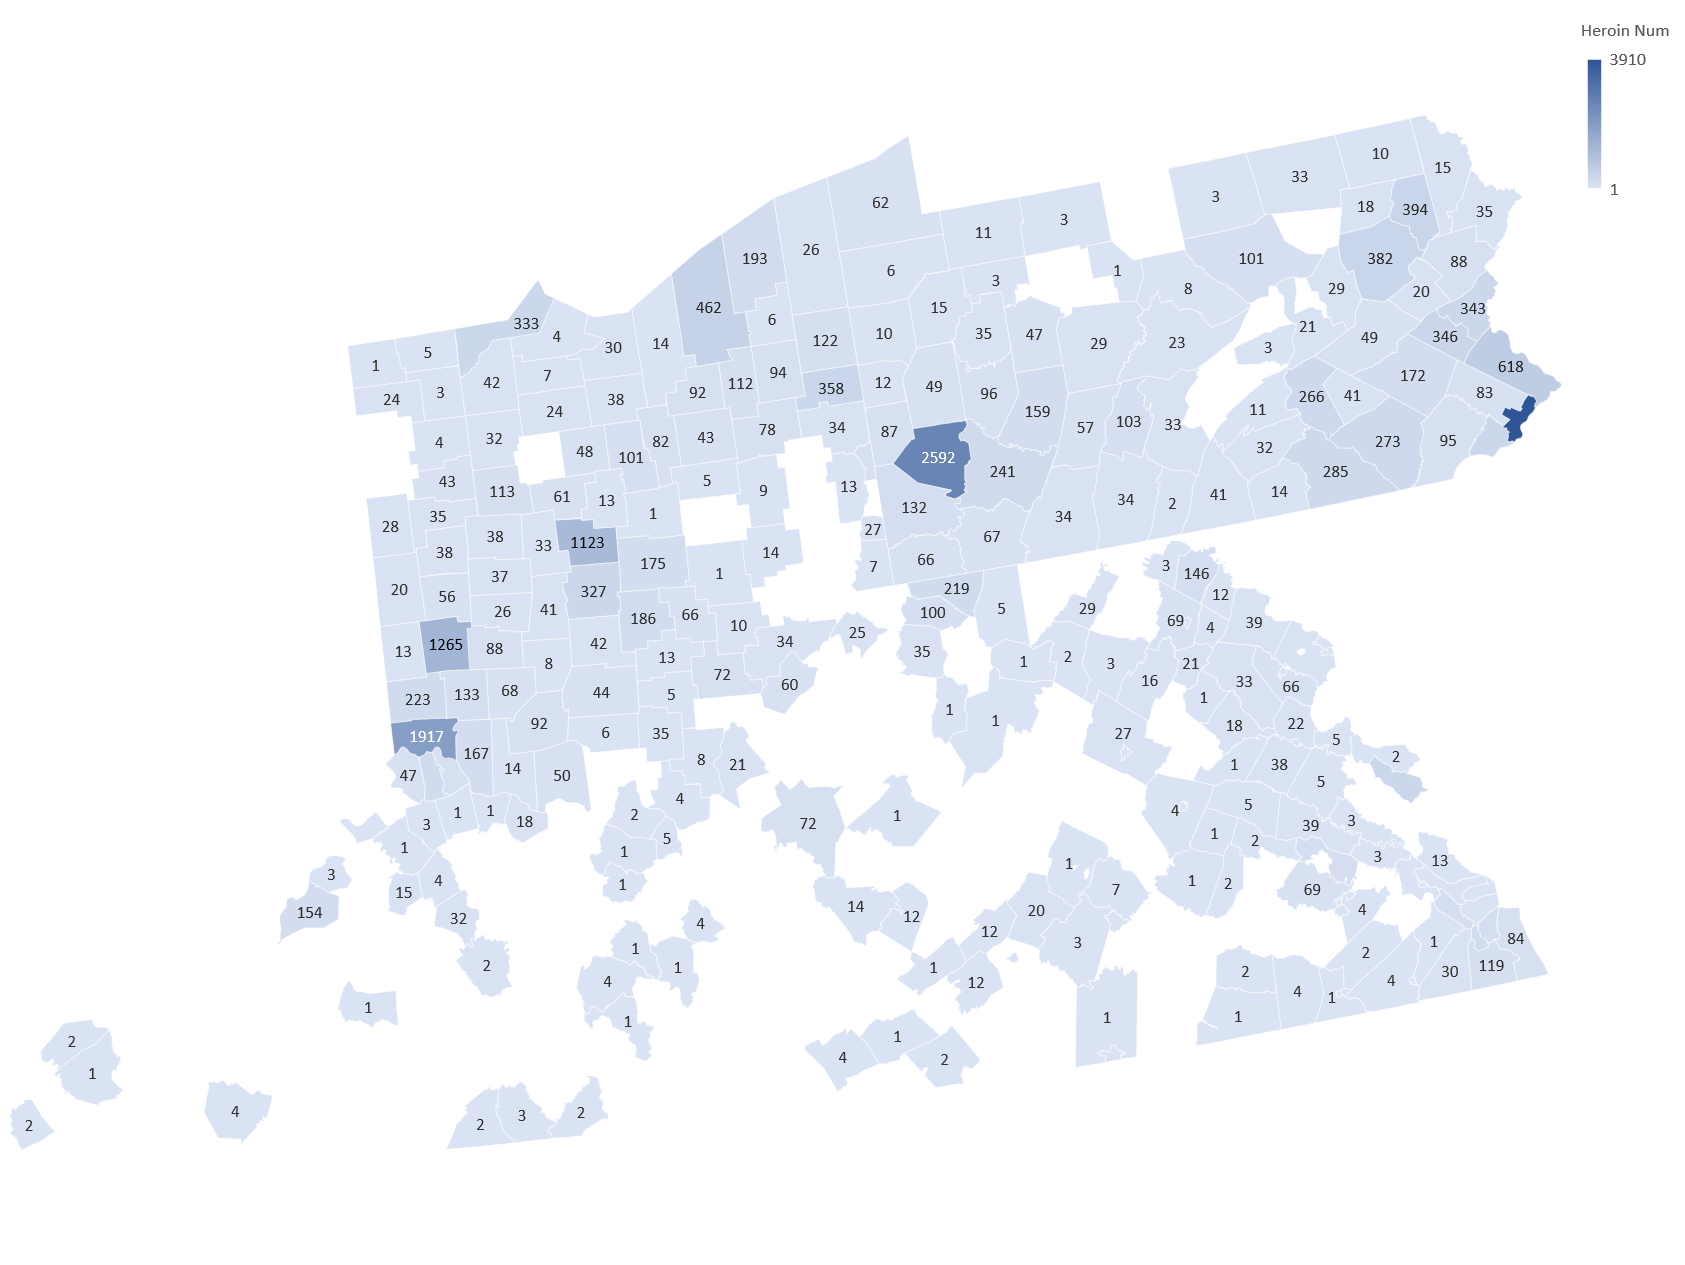
\includegraphics[width = 0.4\textwidth, left]{2010.png}
%     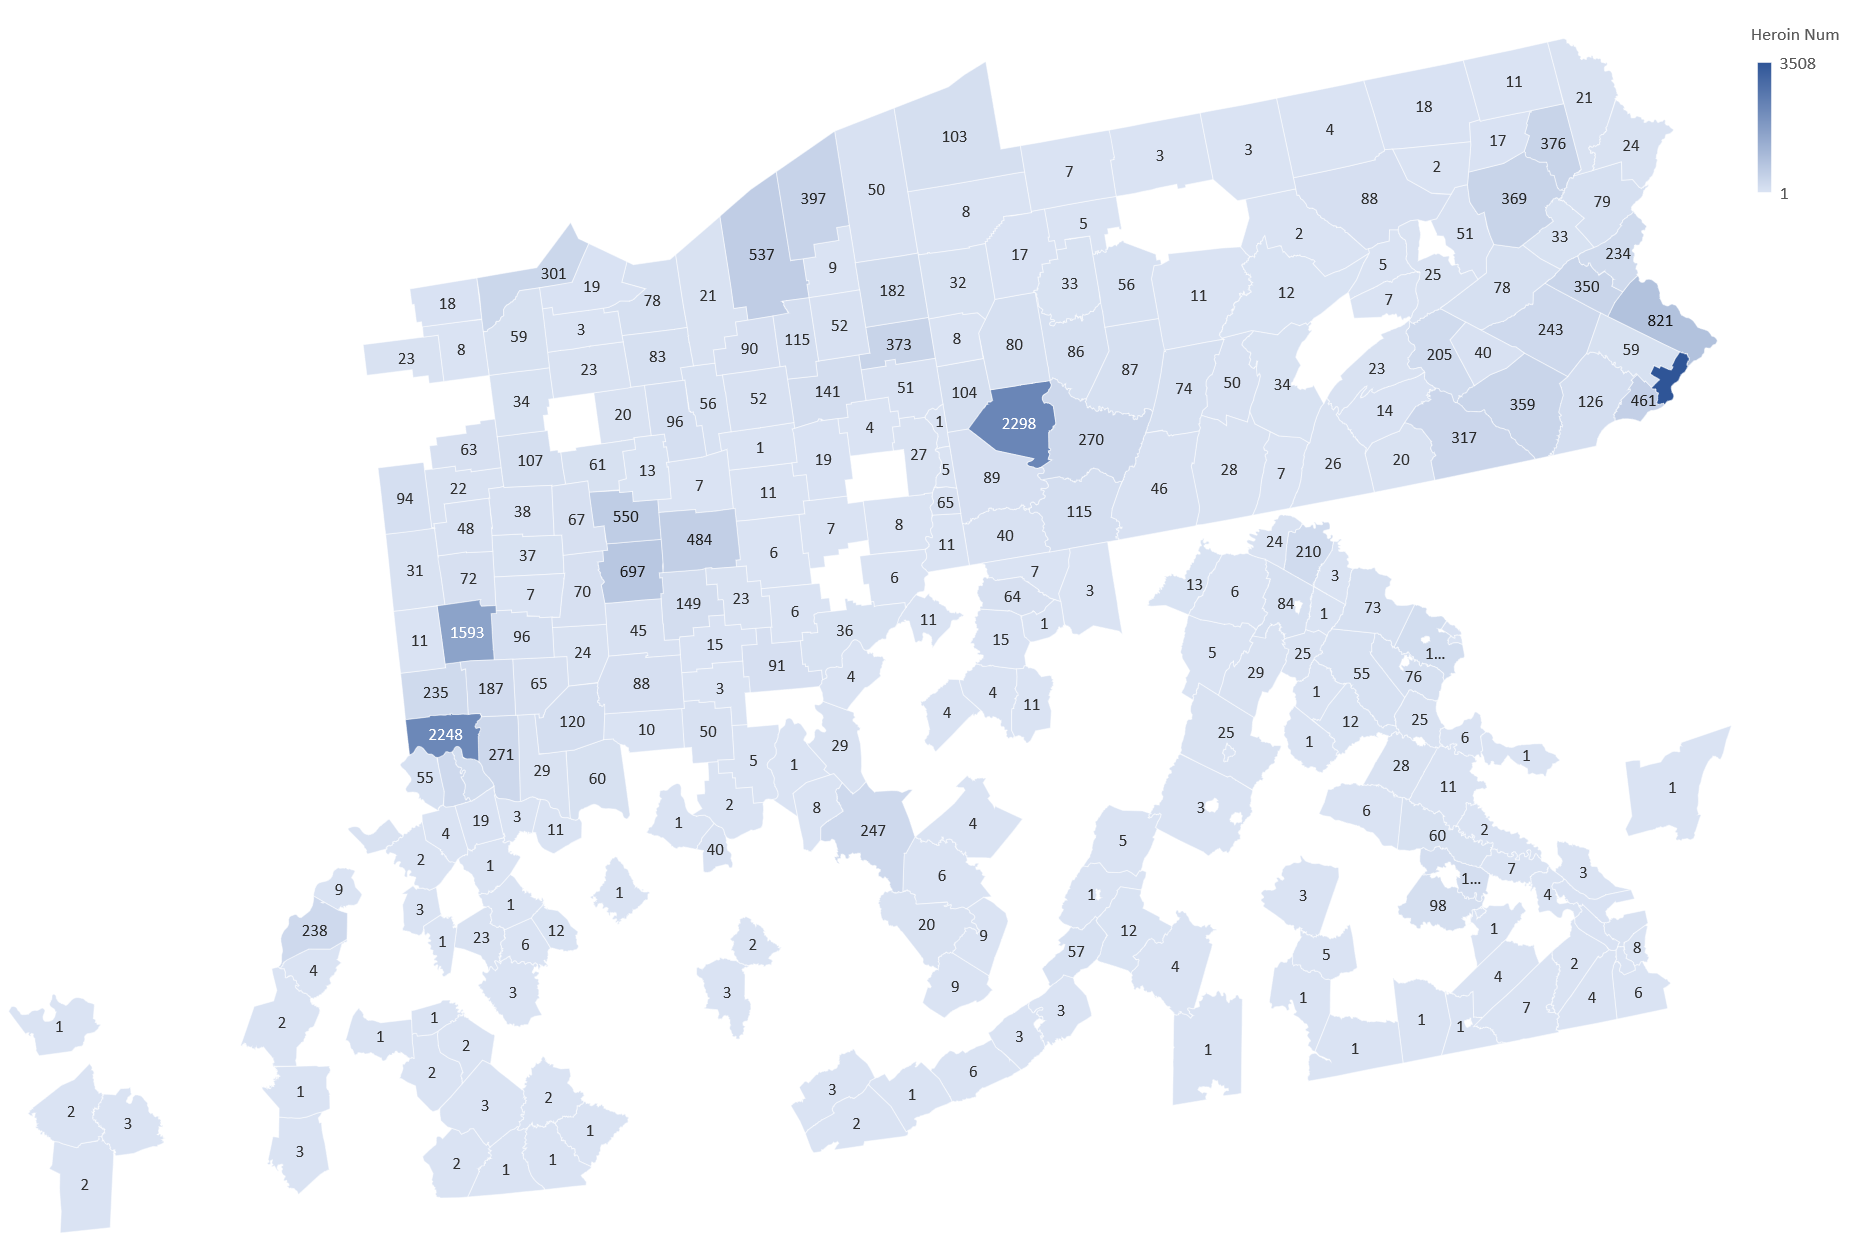
\includegraphics[width = 0.4\textwidth, right]{2011.png}
%     \caption{Caption}
%     \label{fig:my_label}
% \end{figure}

\begin{figure}[H]
   \begin{minipage}{0.48\textwidth}
     \centering
     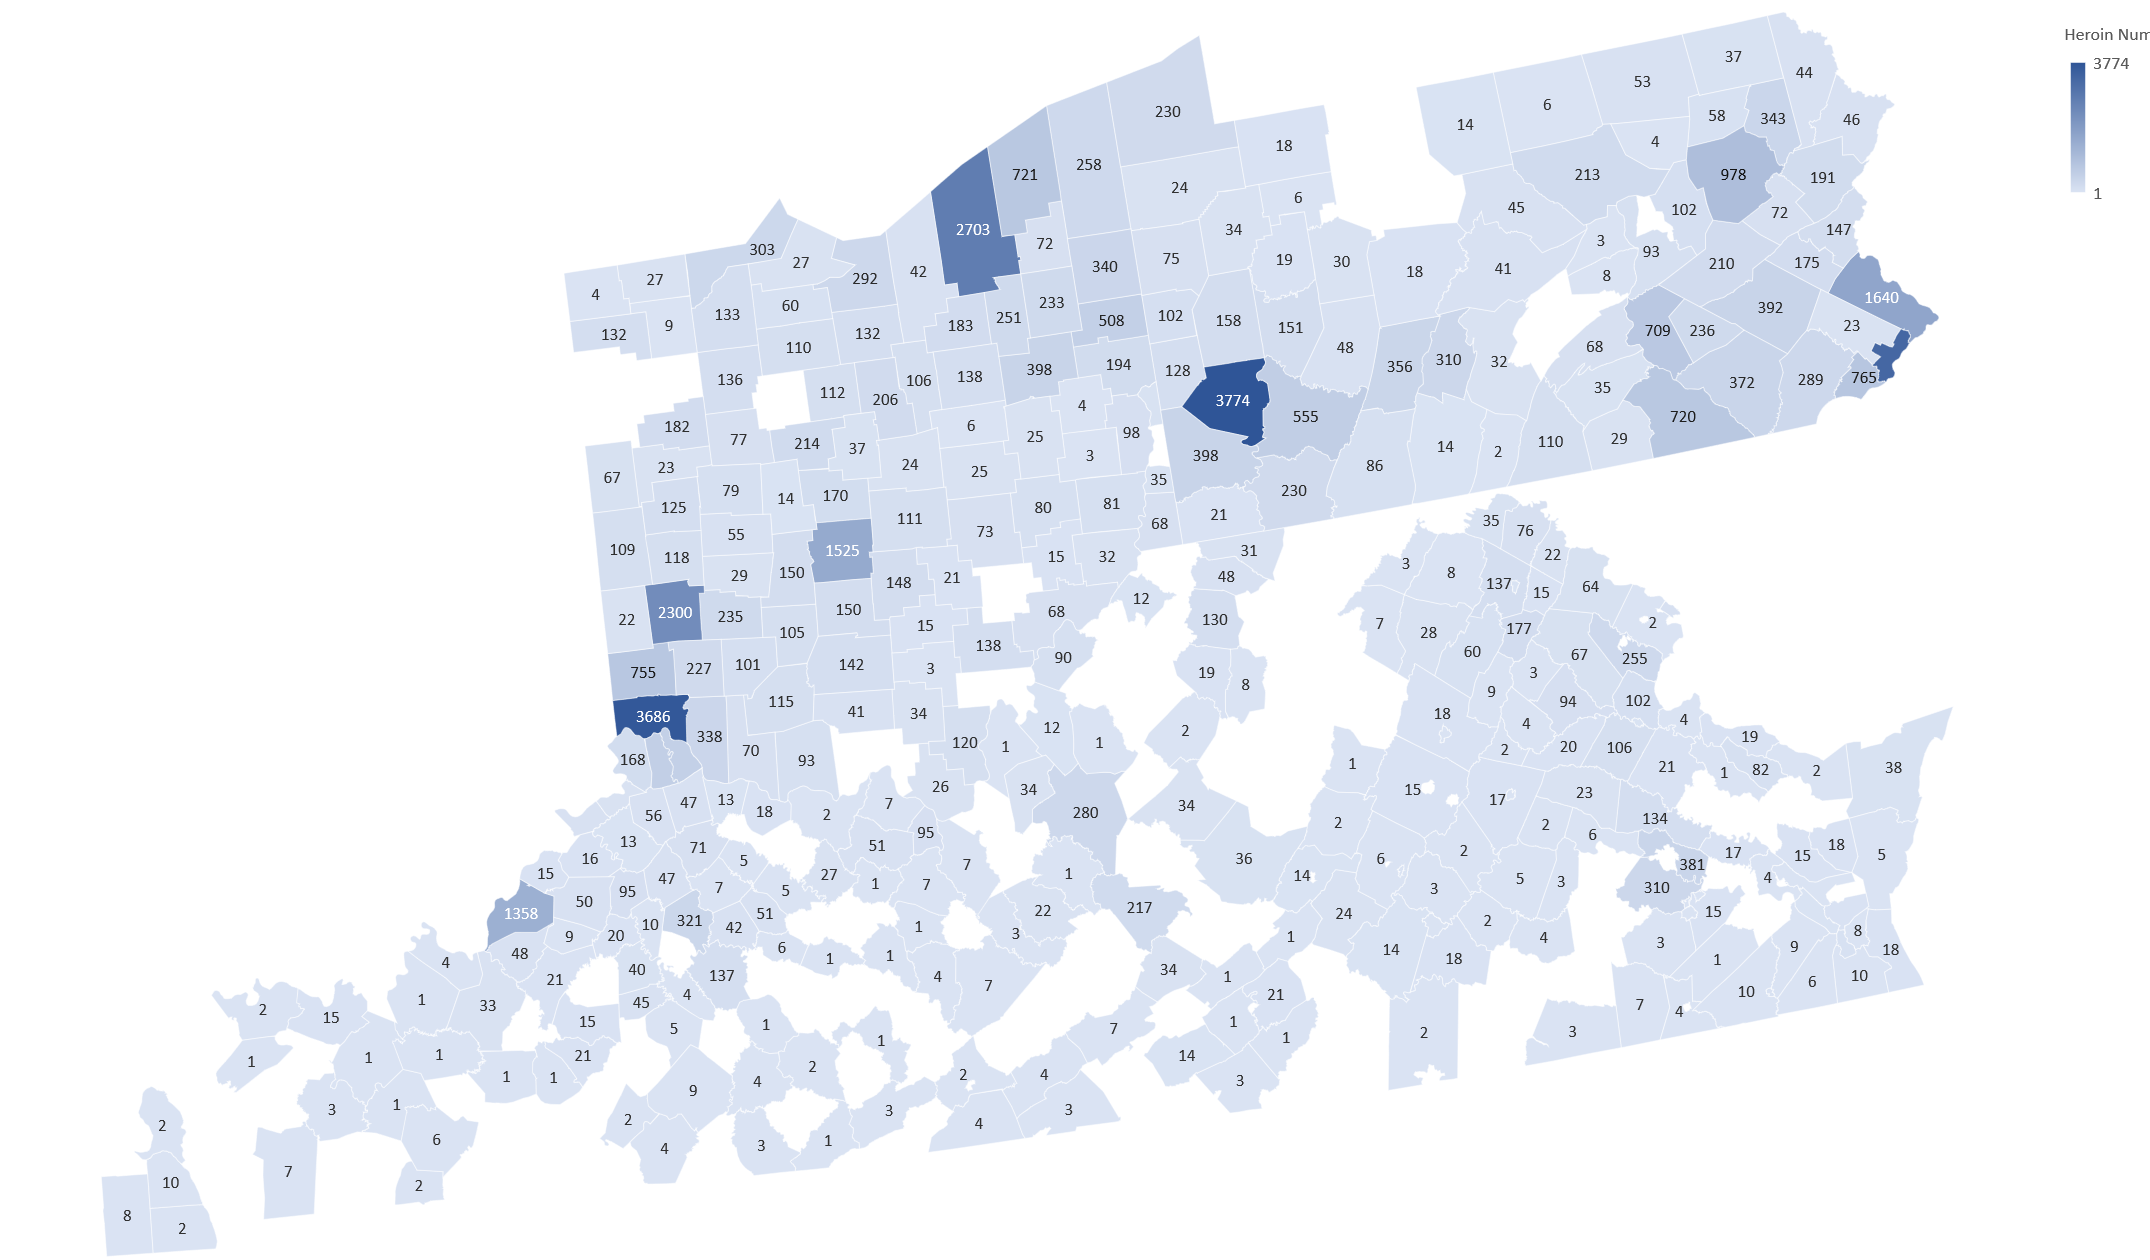
\includegraphics[width=\linewidth]{2014.png}
     \caption{Heroin Reports in 5 states in 2014}\label{H14}
   \end{minipage}%\hfill
   \begin{minipage}{0.48\textwidth}
     \centering
     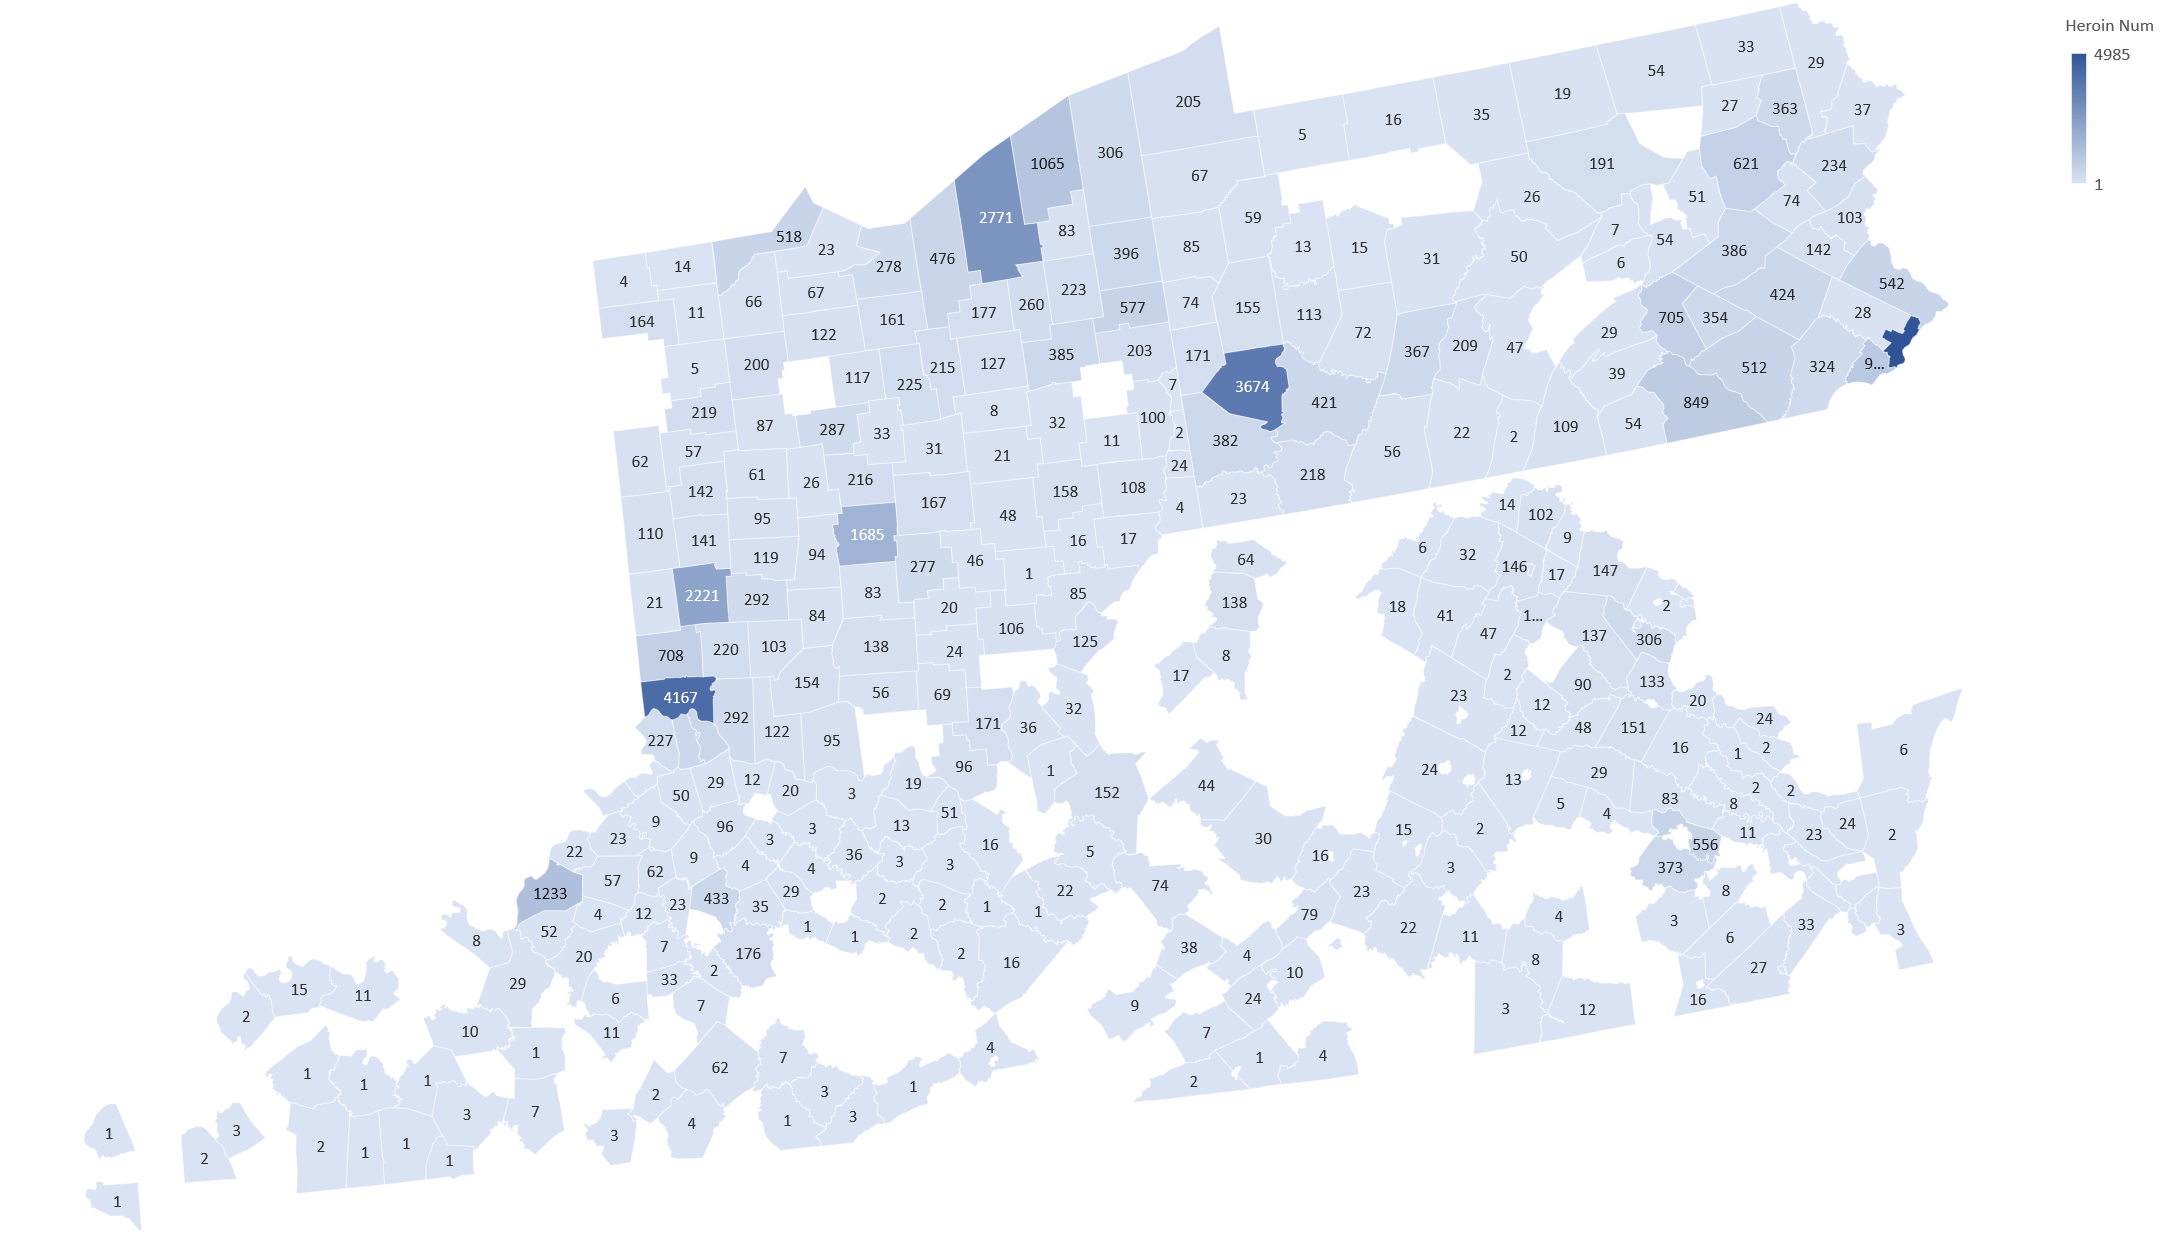
\includegraphics[width=\linewidth]{2015.png}
     \caption{Heroin Reports in 5 states in 2015}\label{H15}
   \end{minipage}
\end{figure}

\begin{figure}[H]
   \begin{minipage}{0.5\textwidth}
     \centering
     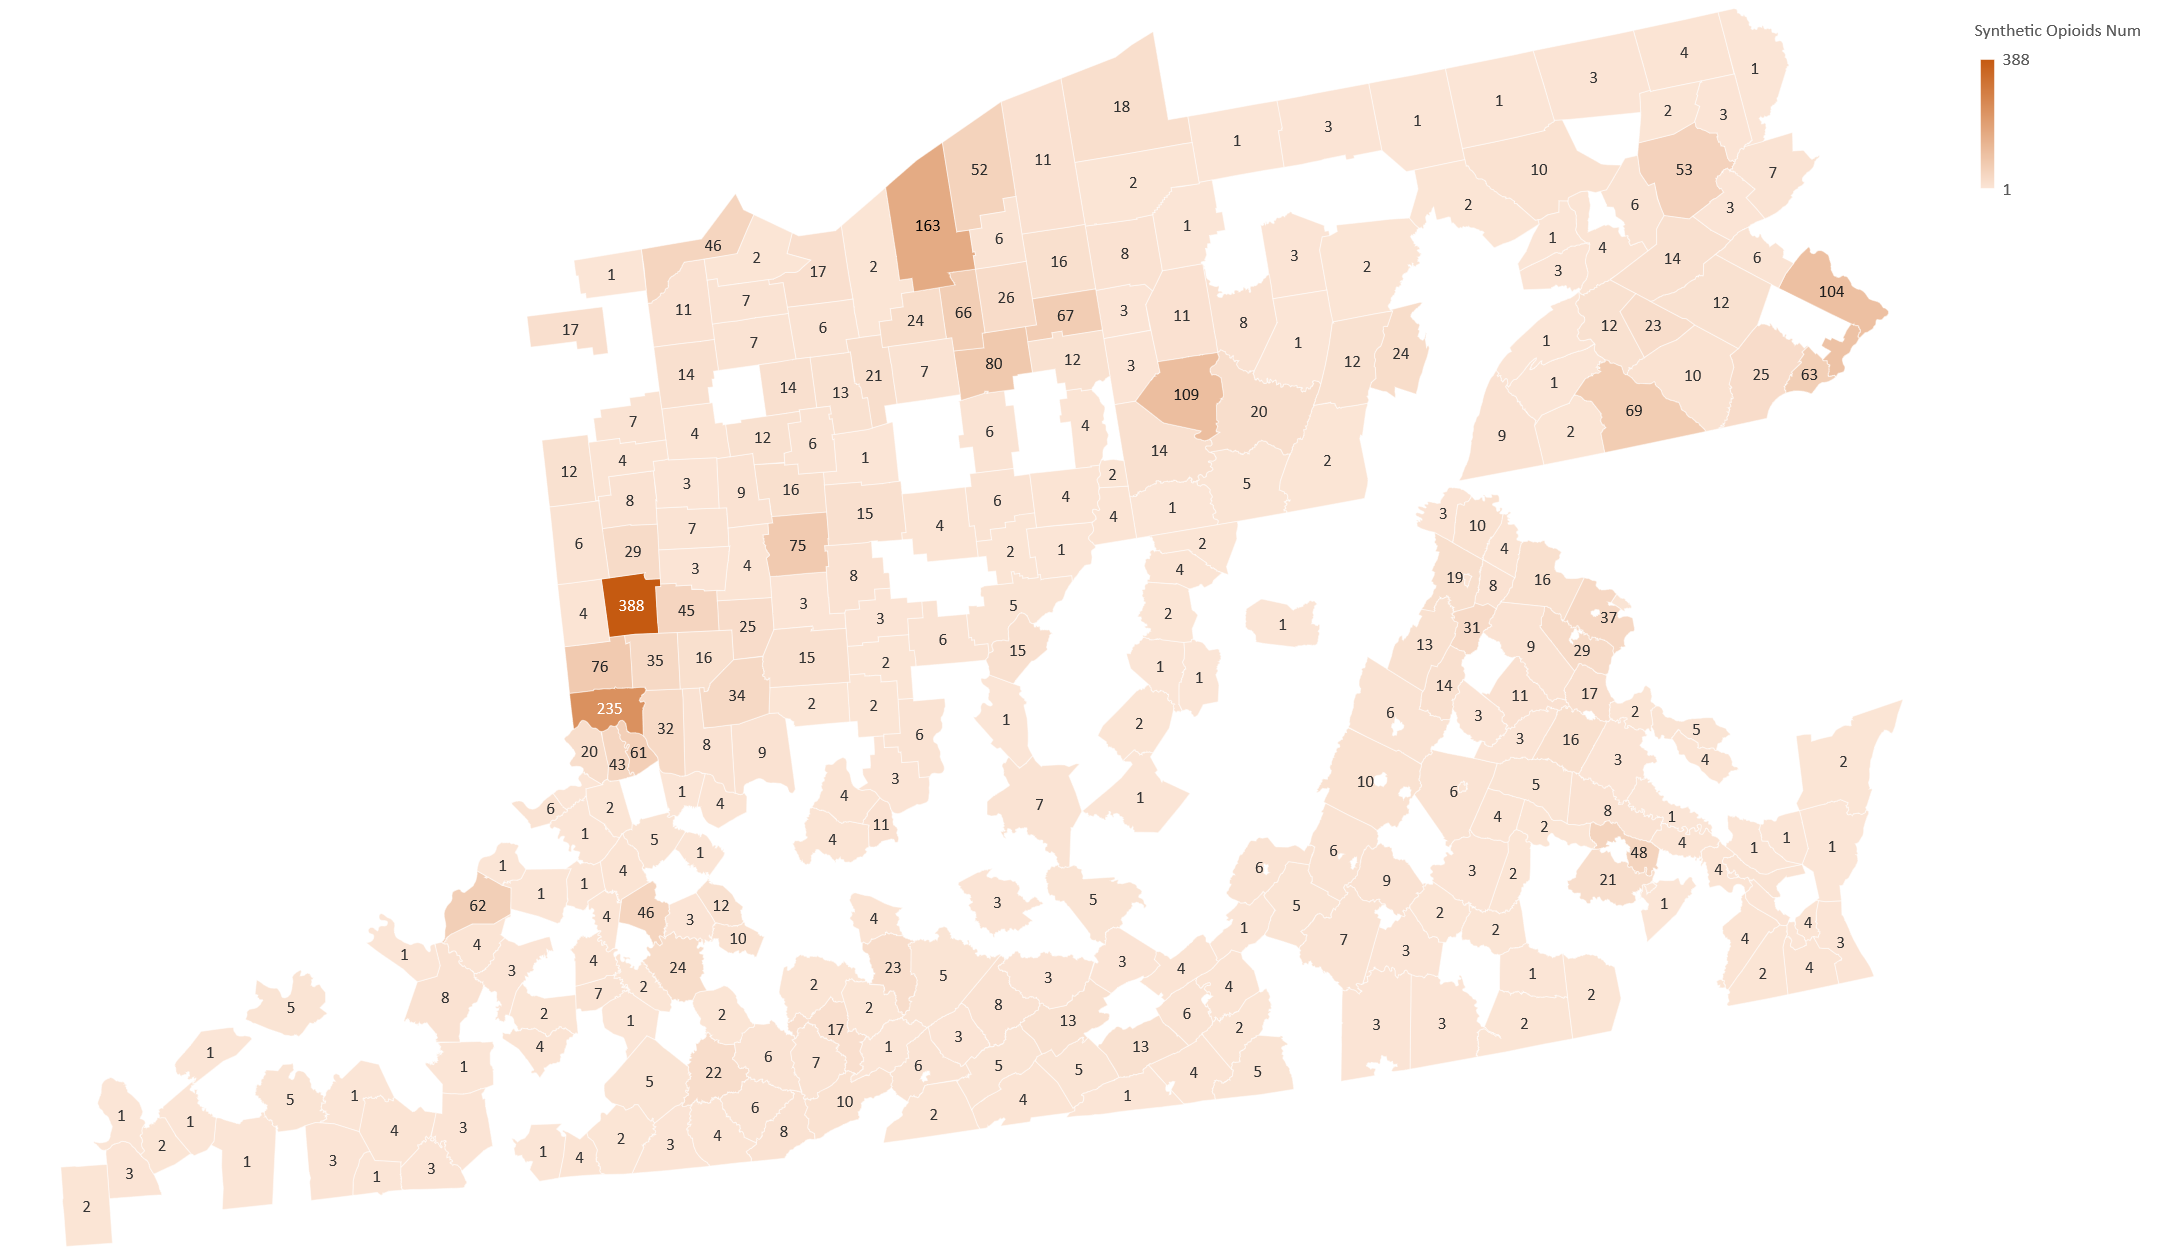
\includegraphics[width=\linewidth]{2014SYN.png}
     \caption{Synthetic Opioid Reports in 5 states in 2014}\label{S14}
   \end{minipage}%\hfill
   \begin{minipage}{0.5\textwidth}
     \centering
     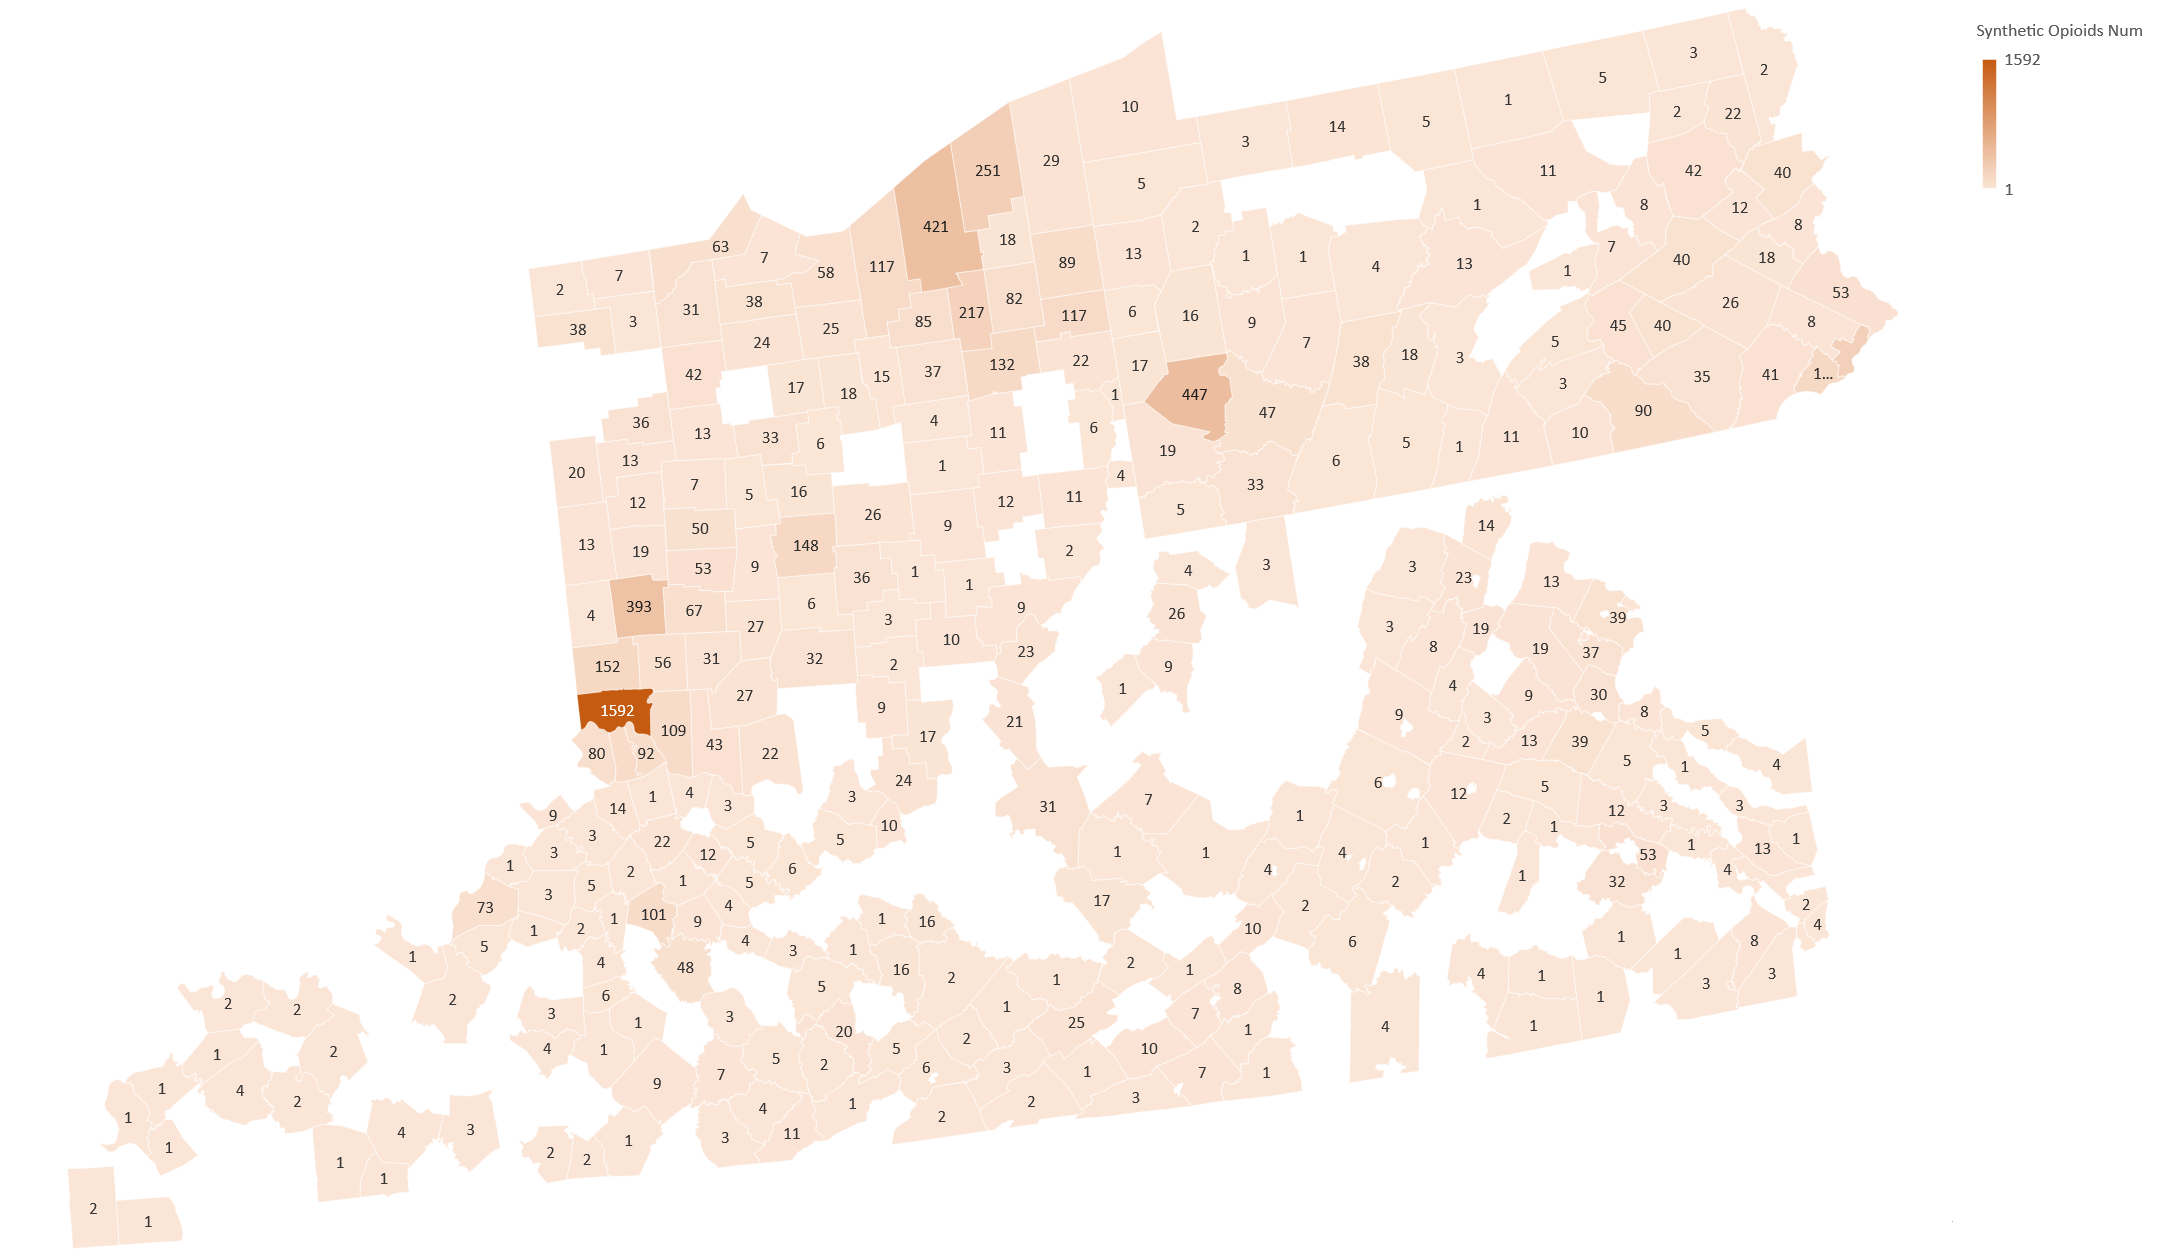
\includegraphics[width=\linewidth]{2015SYN.png}
     \caption{Synthetic Opioid Reports in 5 states in 2014}\label{S15}
   \end{minipage}
\end{figure}

\begin{figure}[H]
   \begin{minipage}{0.5\textwidth}
     \centering
     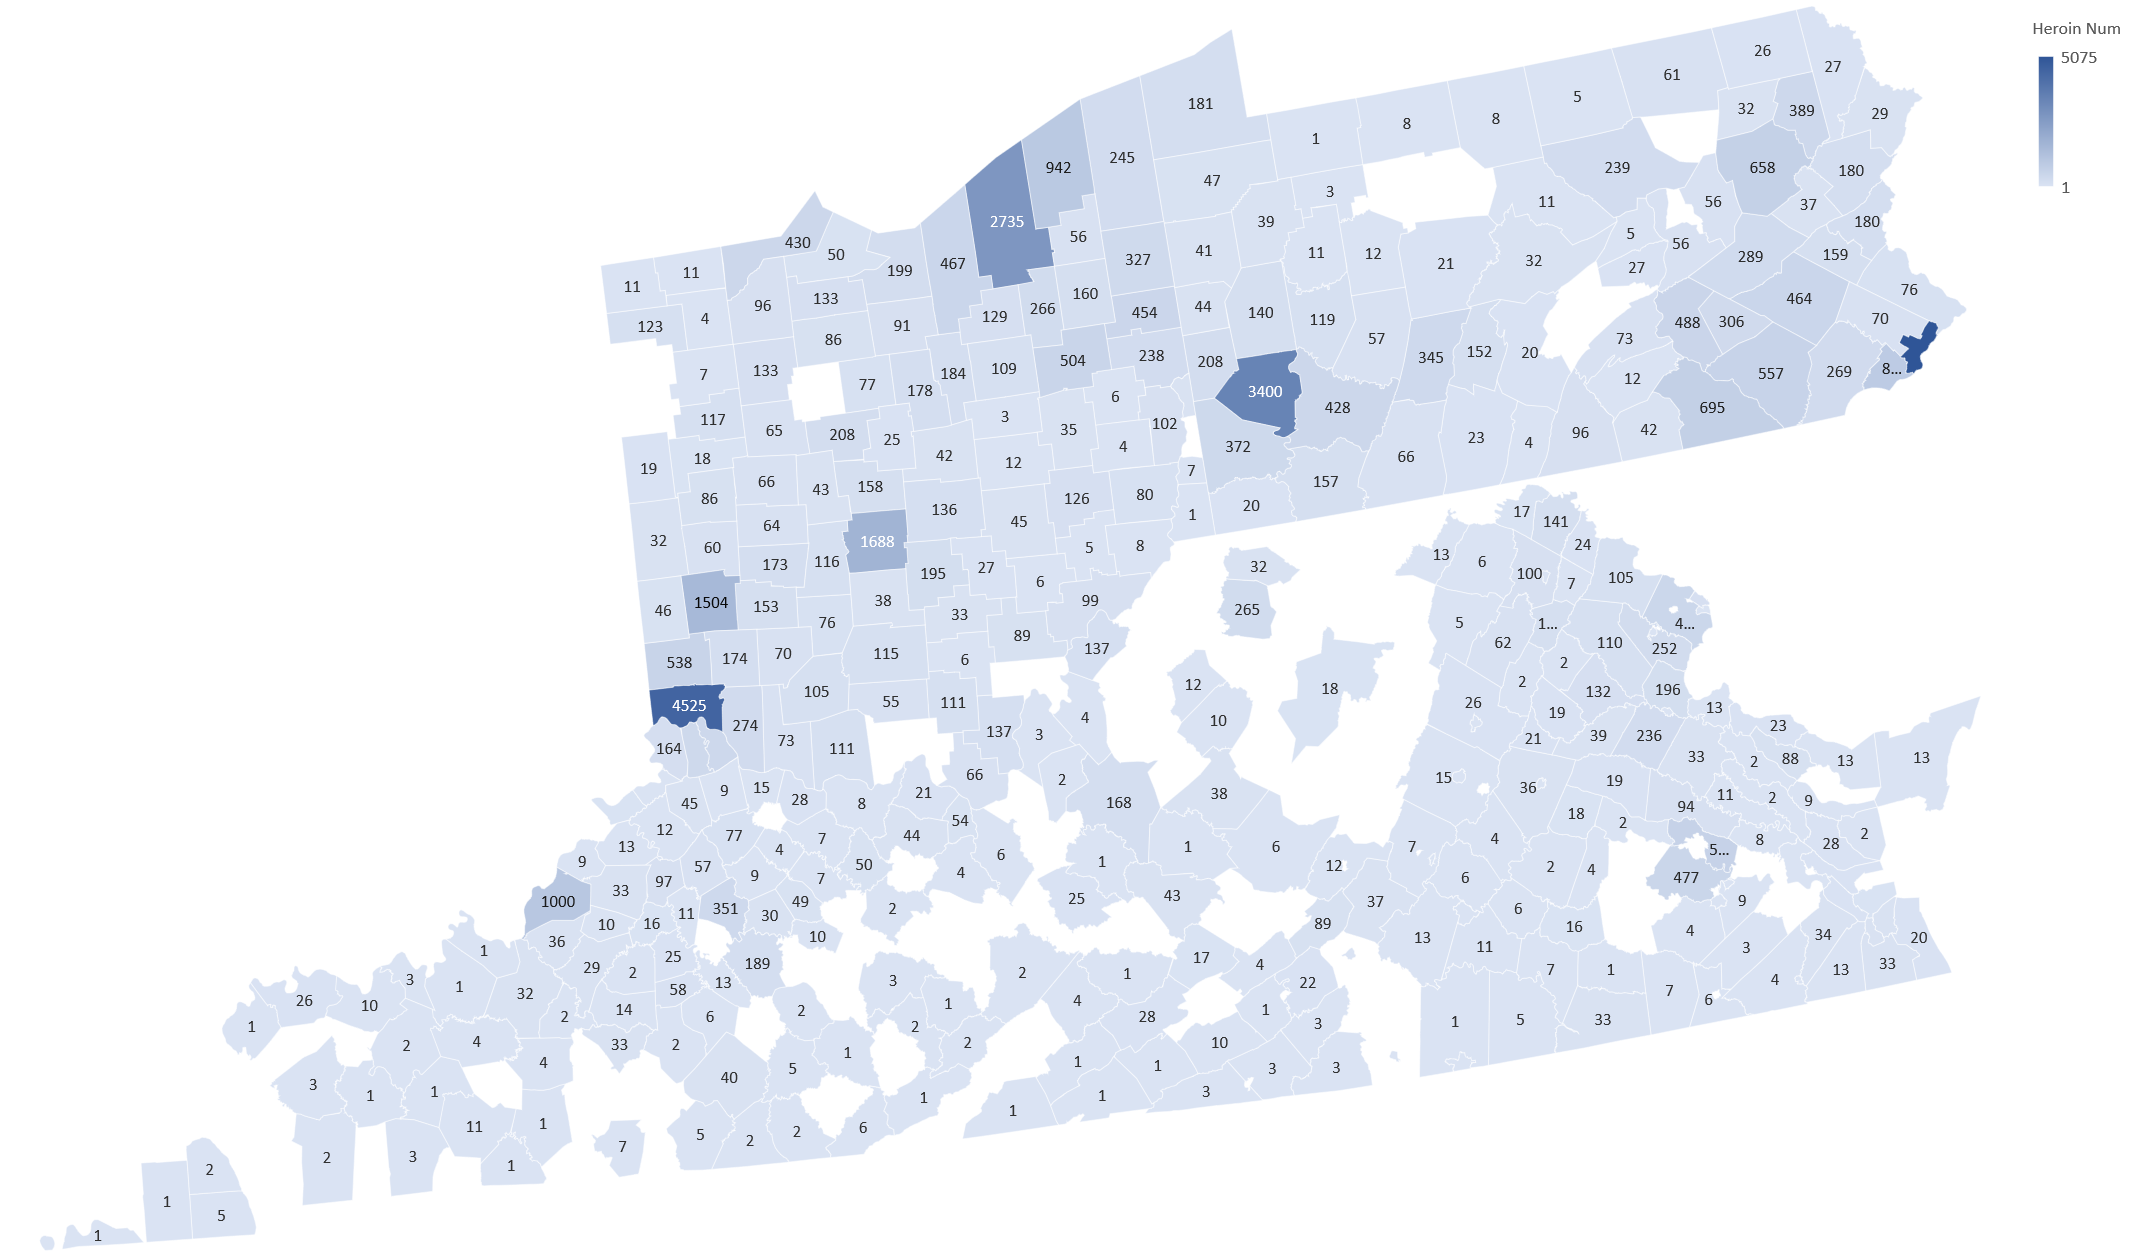
\includegraphics[width=\linewidth]{2016.png}
     \caption{Heroin Reports in 5 states in 2016}\label{H16}
   \end{minipage}%\hfill
   \begin{minipage}{0.5\textwidth}
     \centering
     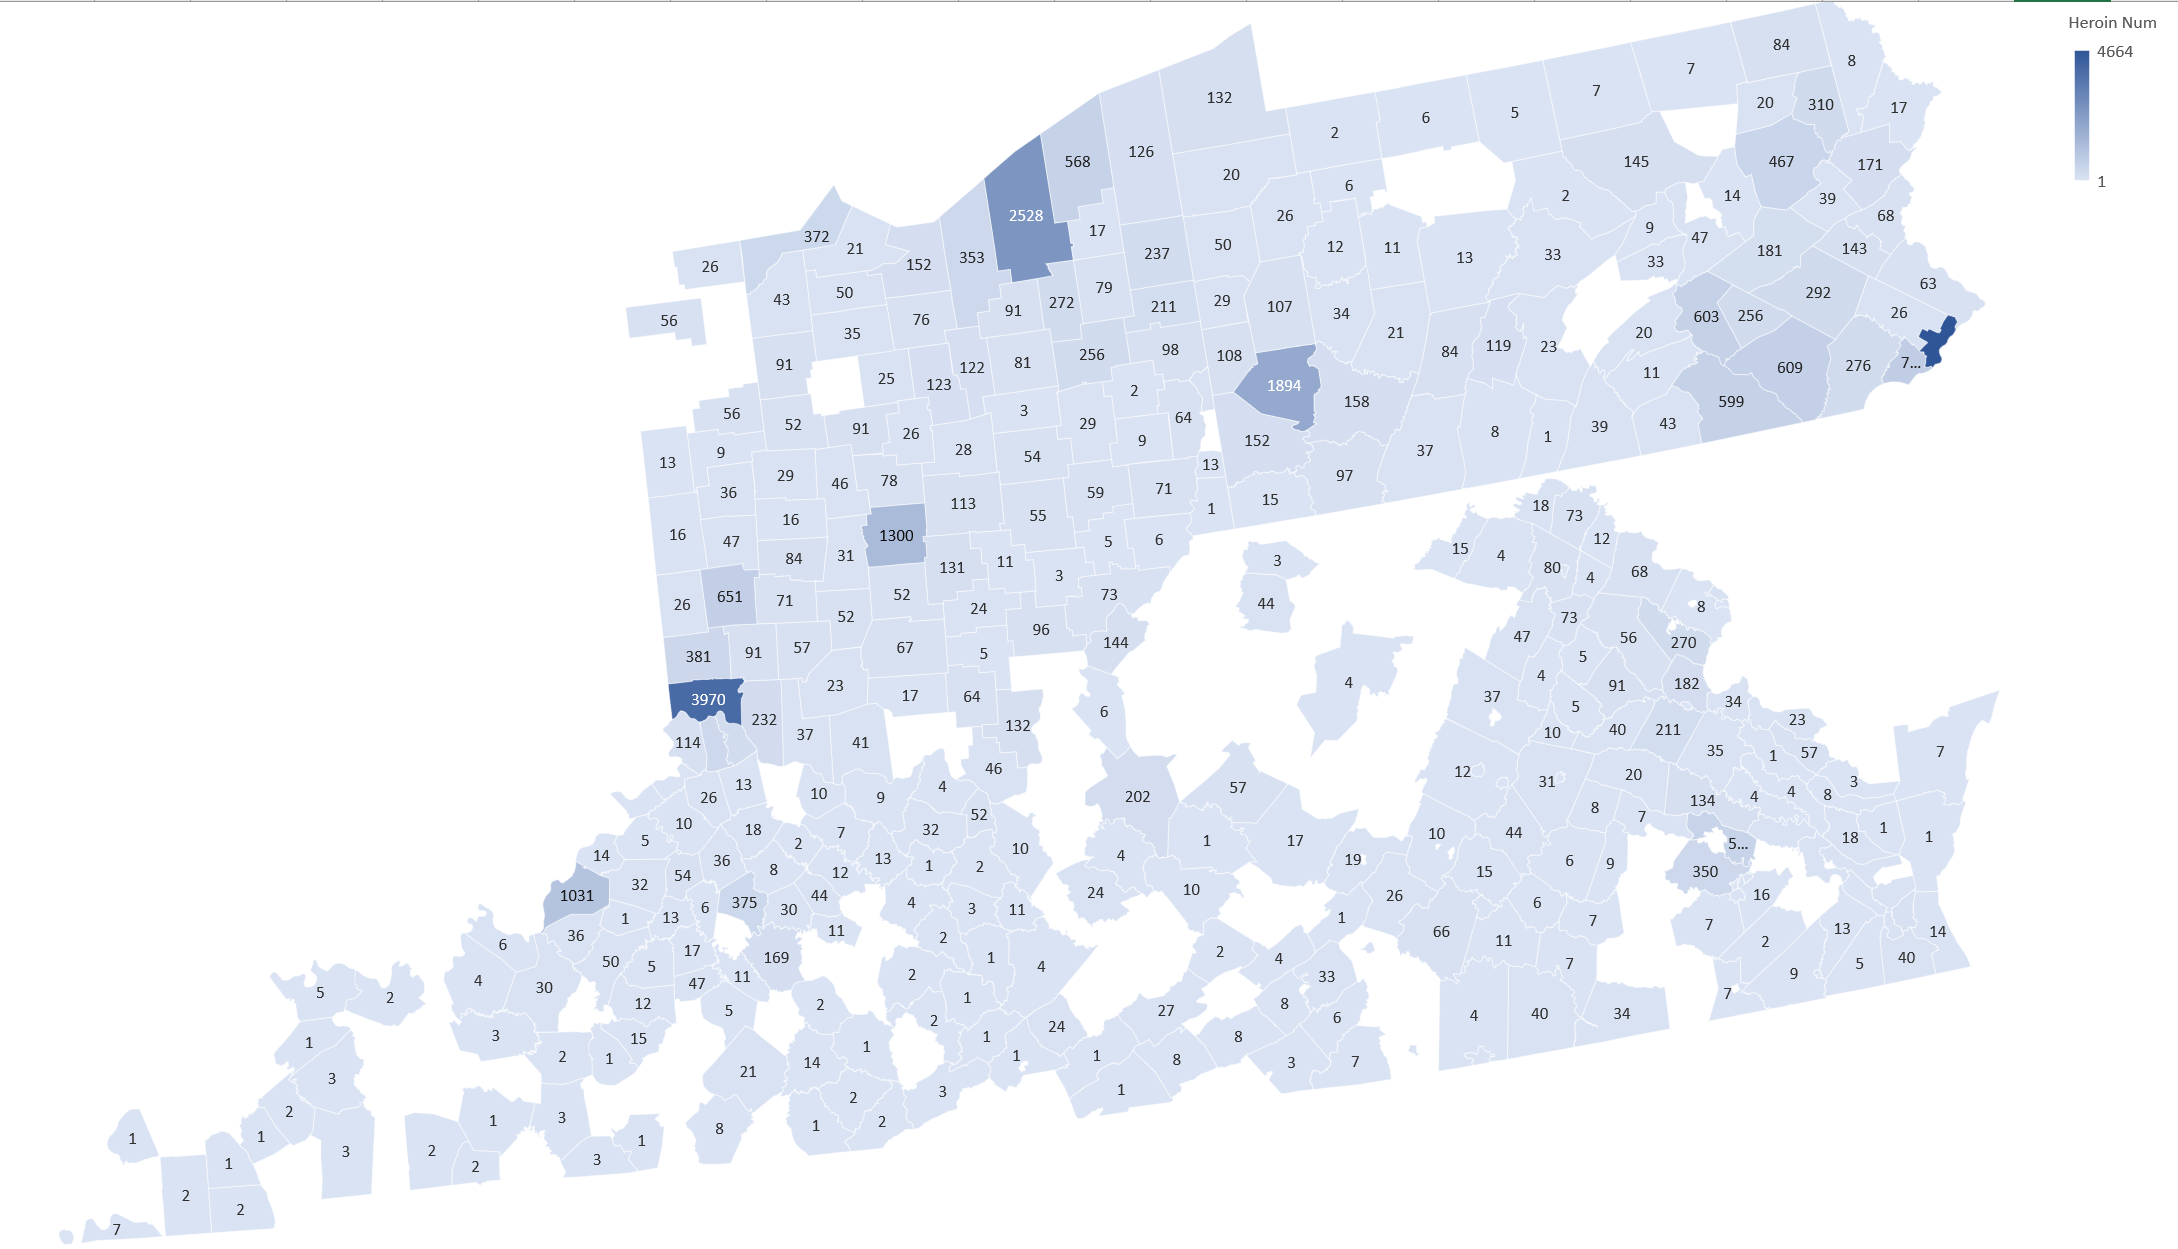
\includegraphics[width=\linewidth]{2017.png}
     \caption{Heroin Reports in 5 states in 2017}\label{H17}
   \end{minipage}
\end{figure}



\begin{figure}[H]
   \begin{minipage}{0.5\textwidth}
     \centering
     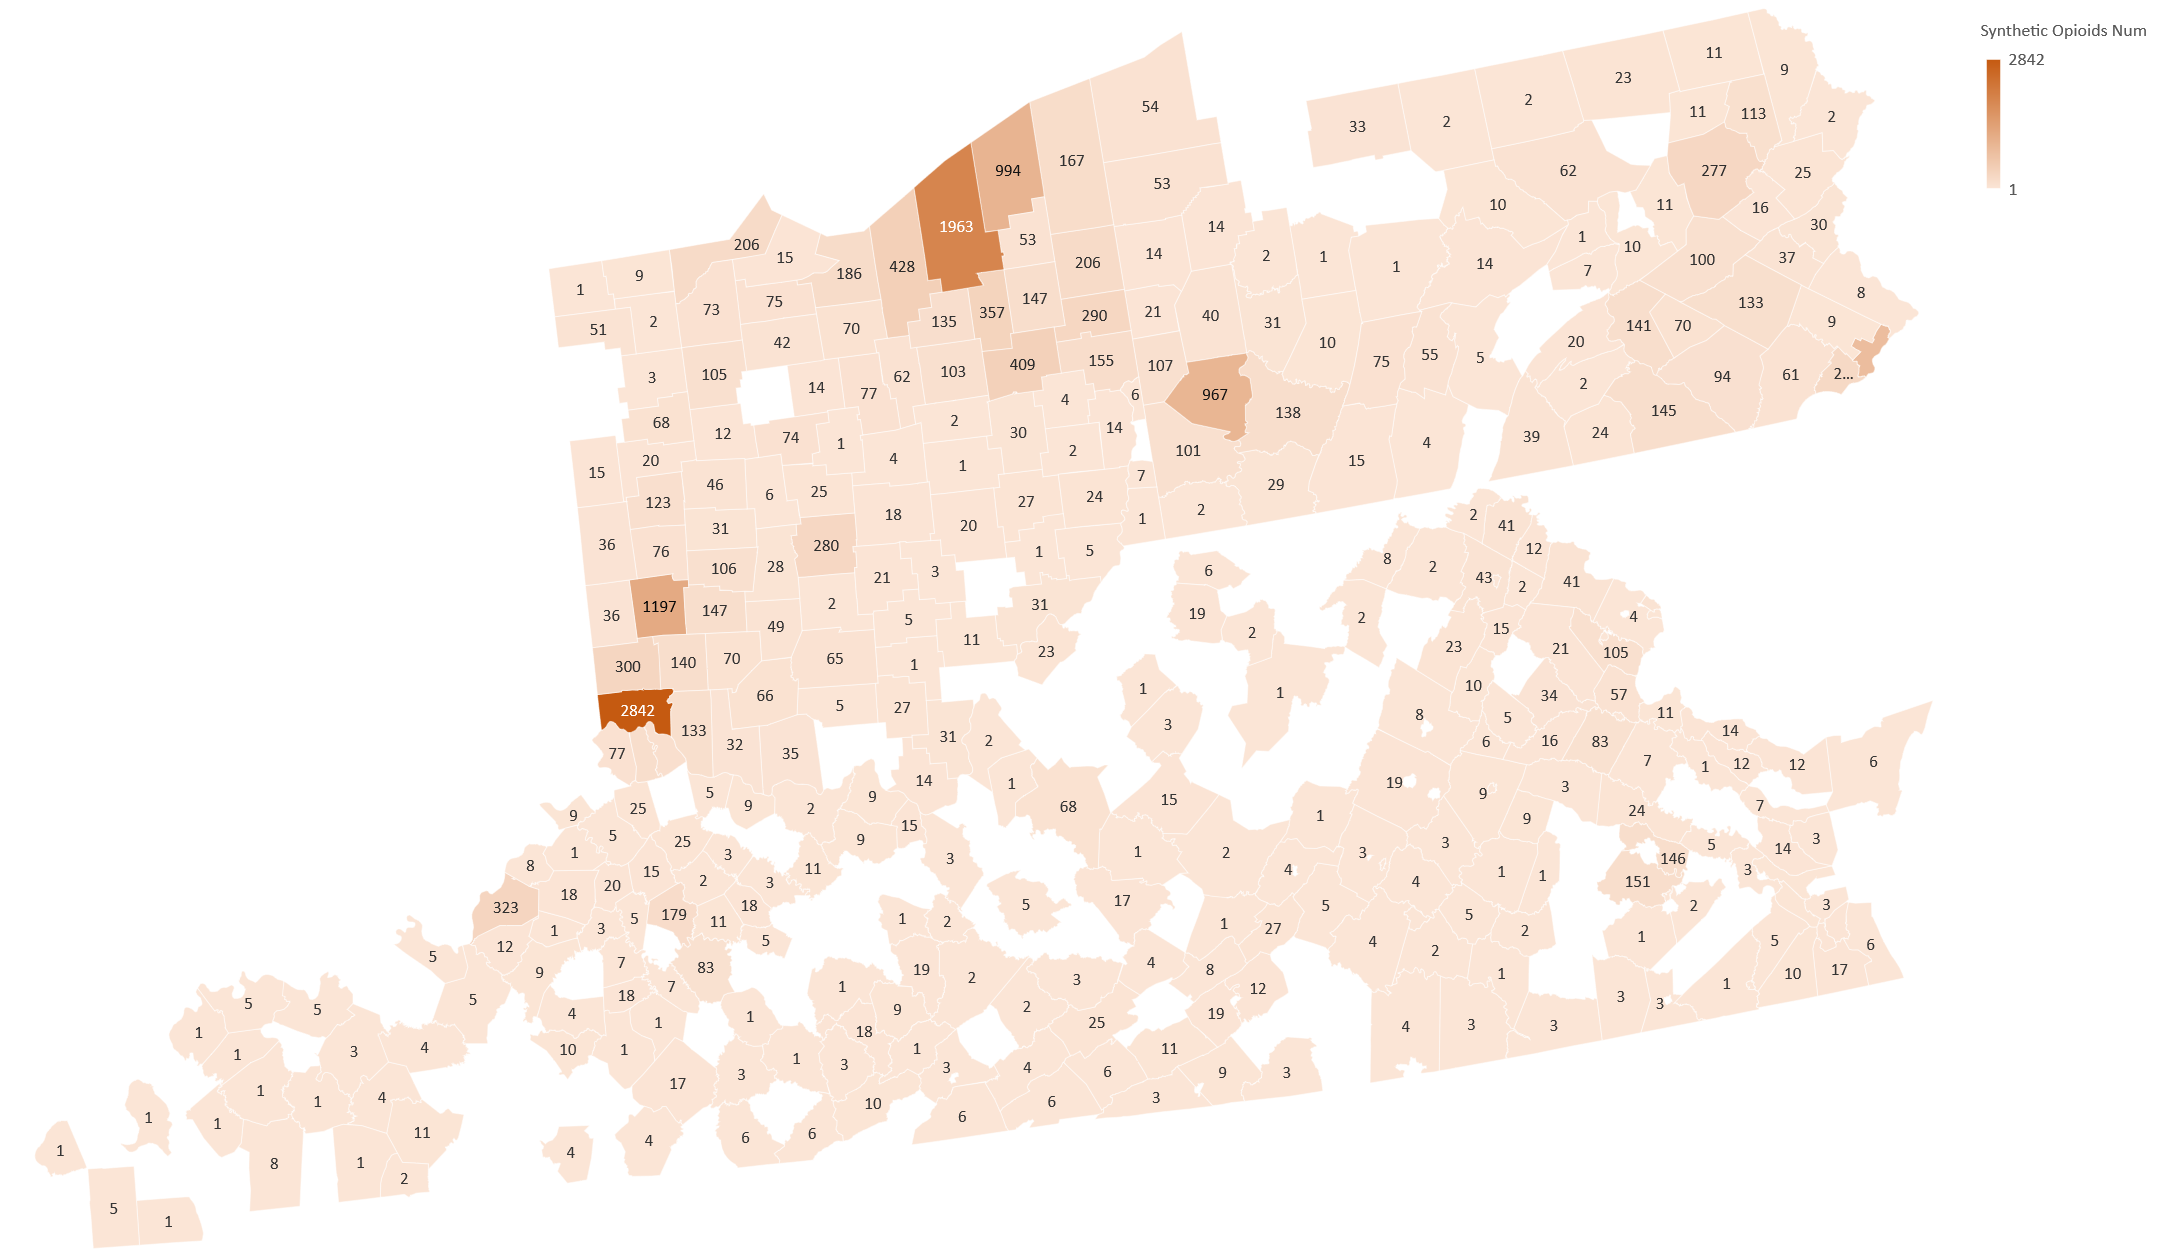
\includegraphics[width=\linewidth]{2016SYN.png}
     \caption{Synthetic Opioid Reports in 5 states in 2014 2016}\label{S16}
   \end{minipage}%\hfill
   \begin{minipage}{0.5\textwidth}
     \centering
     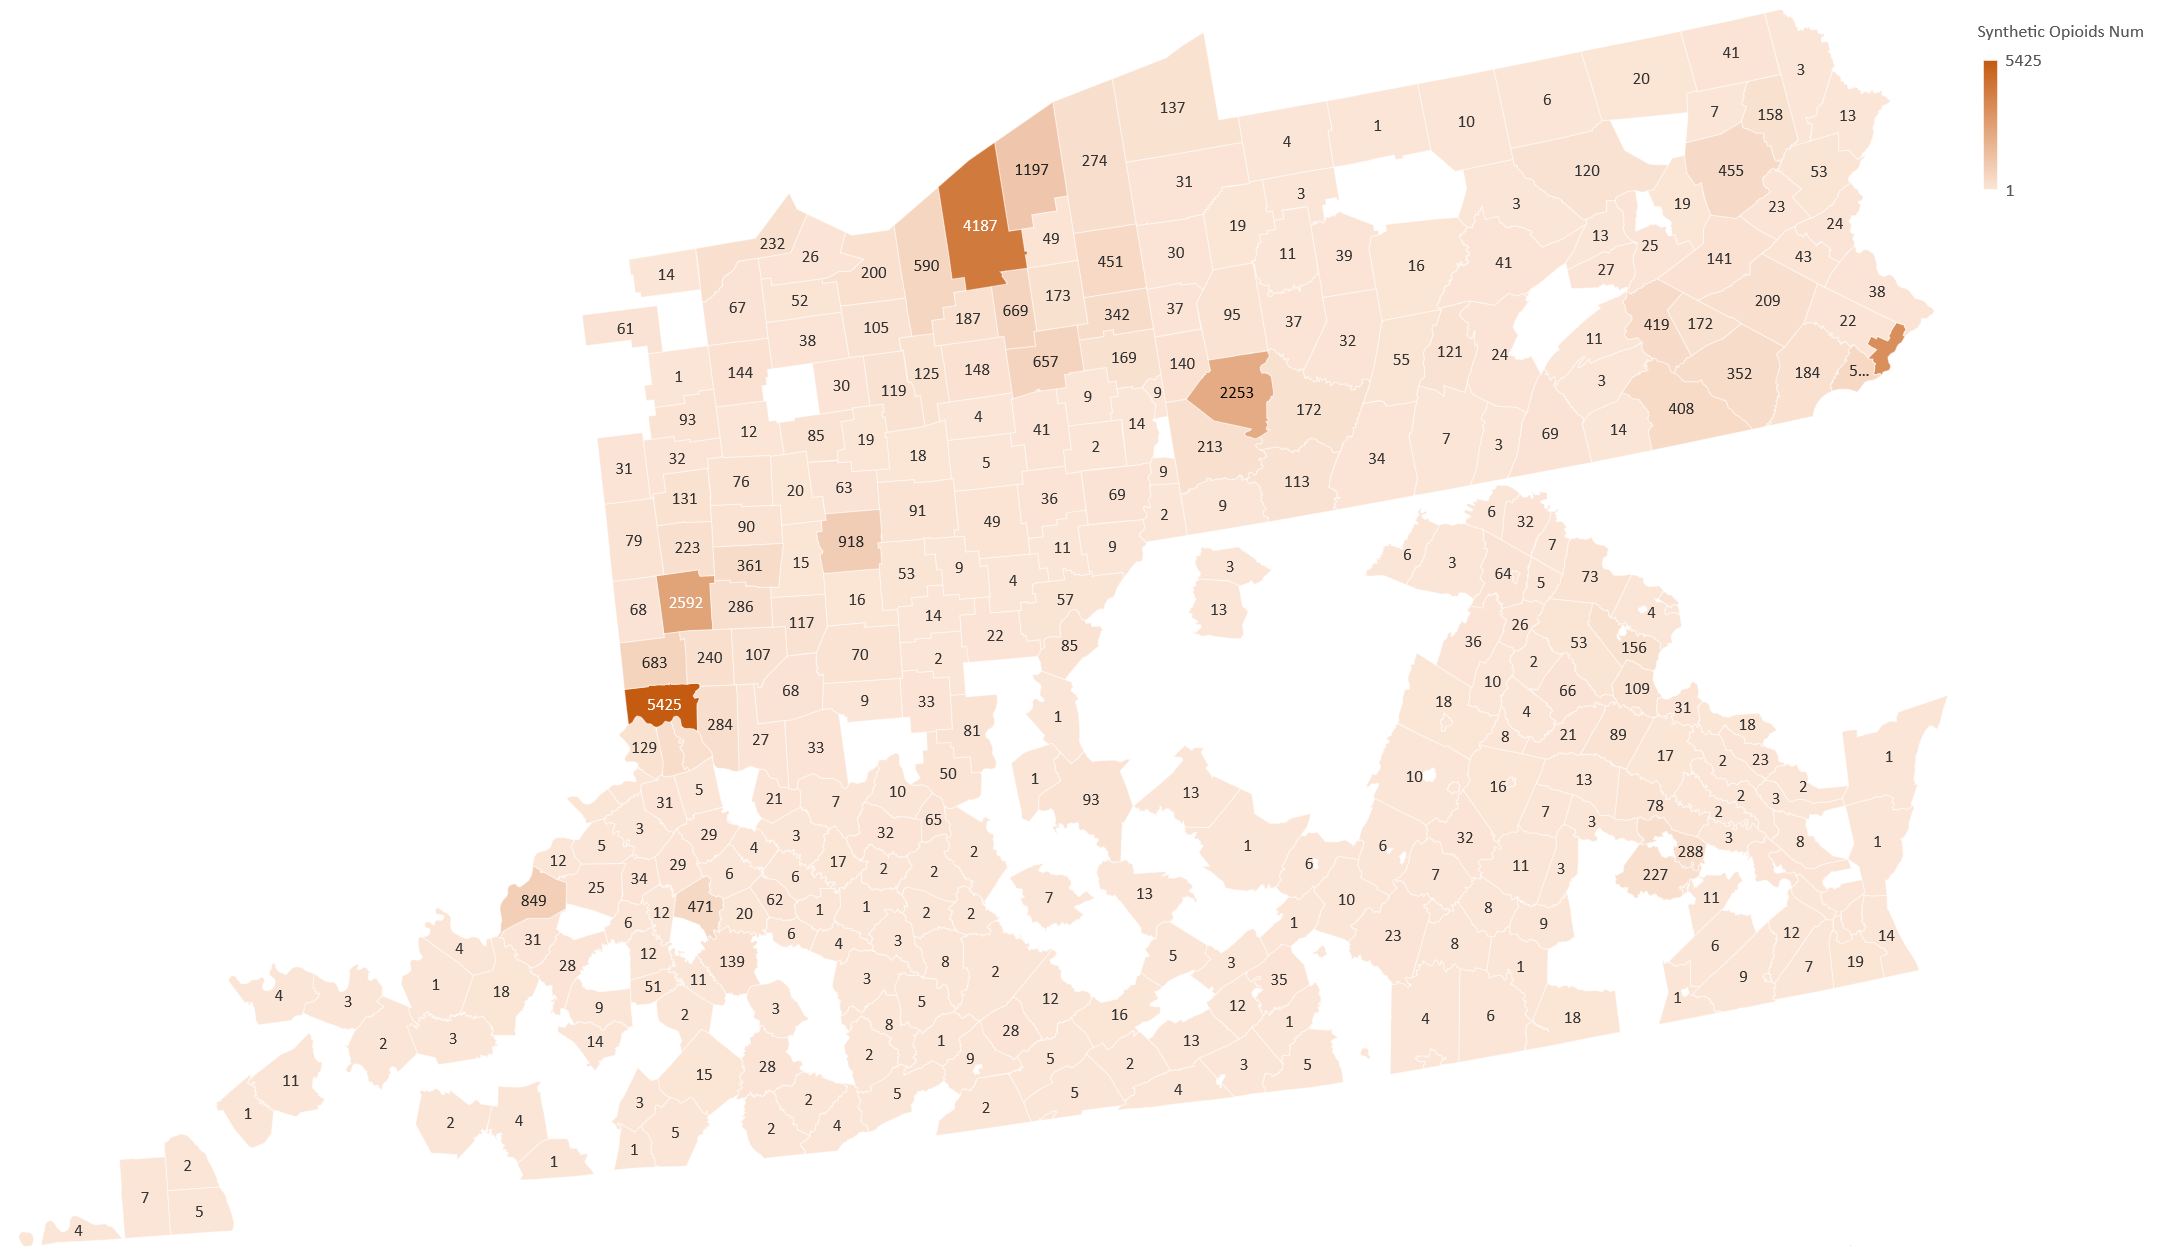
\includegraphics[width=\linewidth]{2017SYN.png}
     \caption{Synthetic Opioid Reports in 5 states in 2014 2017}\label{S17}
   \end{minipage}
\end{figure}


Since according to the data provided, the number of Heroin use reports is constantly increasing roughly at the same rate, we picked pictures by the same time interval (2 years). Yet according to the data provided, the use of synthetic opioids reports grew significantly from year 2014 to year 2015 in Pennsylvania, and then drop down somehow in year 2016, but then rise again in year 2017, so the pictures we showed are chosen specifically for these changes.

\newpage


% - - - - - - - - - - - END Model Design - - - - - - - - - - -



% - - - - - - - - - - - Model Solution - - - - - - - - -

% labels allow you to cross-reference a section later in the document, without having to remember its number
%  - - - - - - - - - - - - - - - - - - - - - - - - - - - - - -
% Delete existing text when writing your own report.


 

% - - - - - - - - - - - END Discussion - - - - - - - - - - -



% - - - - - - - - - - - References - - - - - - - - -
% [1] http://www.comap-math.com/mcm/2019\_MCM-ICM\_Problems.zip


% - - - - - - - - - - - END References - - - - - - - - - - -




% = = = = = = = = = = = = = = = = = = = = = = = = = = = = = = 
%				END YOUR DOCUMENT - did you proofread?
% = = = = = = = = = = = = = = = = = = = = = = = = = = = = = = 
\end{document} % End of document. Nothing after this line will appear in .pdf
% = = = = = = = = = = = = = = = = = = = = = = = = = = = = = = 